\section{OpenQuake Platform connection settings}

\begin{figure}
    \centering
    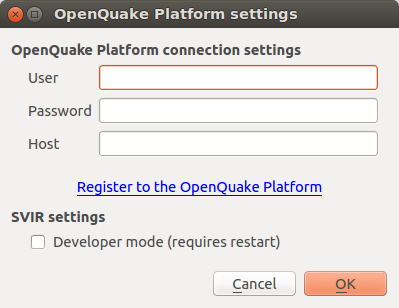
\includegraphics[width=0.8\textwidth]{../images/image07}
    \caption{OQ-Platform connection settings}
    \label{fig:connection_settings}
\end{figure}

Some of the functionalities provided by the plugin, such as the ability to work
with GEM data, require the interaction between the plugin itself and the
OpenQuake Platform (OQ-Platform). The OQ-Platform is a web-based portal to
visualize, explore and share GEM's datasets, tools and models. In the “Platform
Settings” dialog displayed in Figure~\ref{fig:connection_settings}, credentials
must be inserted to authenticate the user and to allow the user to log into the
OQ-Platform. In the ‘Host' field insert the URL of GEM's production
installation of the \href{https://platform.openquake.org}{OQ-Platform} or a
different installation if you have URL access. If you still haven't signed up
to the OQ-Platform, you can do so by clicking `Register to the OQ-Platform'.
This will open a new web browser and
\href{https://platform.openquake.org/account/signup/}{sign up page}.  The
checkbox labeled `Developer mode (requires restart)' can be used to increase
the verbosity of logging. The latter is useful for developers or advanced users
because logging is critical for troubleshooting, but it is not recommended for
standard users.
